\documentclass[a4paper,14pt]{extarticle}

\usepackage[utf8x]{inputenc}
\usepackage[T1]{fontenc}
\usepackage[russian]{babel}
\usepackage{hyperref}
\usepackage{indentfirst}
\usepackage{here}
\usepackage{array}
\usepackage{graphicx}
\usepackage{grffile}
\usepackage{caption}
\usepackage{subcaption}
\usepackage{chngcntr}
\usepackage{amsmath}
\usepackage{amssymb}
\usepackage{pgfplots}
\usepackage{pgfplotstable}
\usepackage[left=2cm,right=2cm,top=2cm,bottom=2cm,bindingoffset=0cm]{geometry}
\usepackage{multicol}
\usepackage{multirow}
\usepackage{titlesec}
\usepackage{listings}
\usepackage{color}
\usepackage{longtable}
\usepackage{enumitem}
\usepackage{cmap}
\usepackage{tikz}

\usetikzlibrary{shapes,arrows}

\definecolor{green}{rgb}{0,0.6,0}
\definecolor{gray}{rgb}{0.5,0.5,0.5}
\definecolor{purple}{rgb}{0.58,0,0.82}

\lstset{
	language={Java},
	inputpath={../../},
	backgroundcolor=\color{white},
	commentstyle=\color{green},
	keywordstyle=\color{blue},
	numberstyle=\scriptsize\color{gray},
	stringstyle=\color{purple},
	basicstyle=\tiny,
	breakatwhitespace=false,
	breaklines=true,
	captionpos=b,
	keepspaces=true,
	numbers=left,
	numbersep=5pt,
	showspaces=false,
	showstringspaces=false,
	showtabs=false,
	tabsize=8,
	frame=single,
}

\renewcommand{\le}{\ensuremath{\leqslant}}
\renewcommand{\leq}{\ensuremath{\leqslant}}
\renewcommand{\ge}{\ensuremath{\geqslant}}
\renewcommand{\geq}{\ensuremath{\geqslant}}
\renewcommand{\epsilon}{\ensuremath{\varepsilon}}
\renewcommand{\phi}{\ensuremath{\varphi}}
\renewcommand{\thefigure}{\arabic{figure}}
\def\code#1{\texttt{#1}}

\titleformat*{\section}{\large\bfseries} 
\titleformat*{\subsection}{\normalsize\bfseries} 
\titleformat*{\subsubsection}{\normalsize\bfseries} 
\titleformat*{\paragraph}{\normalsize\bfseries} 
\titleformat*{\subparagraph}{\normalsize\bfseries} 

\counterwithin{figure}{section}
\counterwithin{equation}{section}
\counterwithin{table}{section}
\newcommand{\sign}[1][5cm]{\makebox[#1]{\hrulefill}}
\newcommand{\equipollence}{\quad\Leftrightarrow\quad}
\newcommand{\no}[1]{\overline{#1}}
\graphicspath{{figs/}}
\captionsetup{justification=centering,margin=1cm}
\def\arraystretch{1.3}
\setlength\parindent{5ex}
\titlelabel{\thetitle.\quad}

\setitemize{itemsep=0em}
\setenumerate{itemsep=0em}

\tikzstyle{startstop} = [
	rectangle,
	align=center,
	rounded corners,
	text width=10em,
	text centered,
	draw=black
]
\tikzstyle{process} = [
	rectangle,
	align=center,
	text width=20em,
	text centered,
	draw=black
]
\tikzstyle{decision} = [
	diamond,
	aspect=4,
	align=center,
	inner sep=0pt,
	text width=10em,
	text centered,
	node distance=5em,
	draw=black
]
\tikzstyle{line} = [
	draw=black,
	thick,
	->,
	>=stealth,
	-latex'
]

\begin{document}

\begin{titlepage}
\begin{center}
	САНКТ-ПЕТЕРБУРГСКИЙ ПОЛИТЕХНИЧЕСКИЙ УНИВЕРСИТЕТ\\ ПЕТРА ВЕЛИКОГО\\[0.3cm]
	\par\noindent\rule{10cm}{0.4pt}\\[0.3cm]
	Институт компьютерных наук и технологий \\[0.3cm]
	Кафедра компьютерных систем и программных технологий\\[4cm]
	
	Отчет по лабораторной работе\\[3mm]
	Дисциплина: <<Тестирование программного обеспечения>>\\[3mm]
	Тема: <<Тестирование реализации протокола XMPP>>\\[7cm]
\end{center}

\begin{flushleft}
	\hspace*{5mm} Выполнил студент гр. 43501/3  \hspace*{2.5cm}\sign[3cm]\hfill А.Ю. Ламтев\\
	\hspace*{10.4cm} (подпись)\\[3mm]
	\hspace*{5mm} Преподаватель \hspace*{6.0cm}\sign[3cm]\hfill М.Х. Ахин\\
	\hspace*{10.4cm} (подпись)\\[3mm]
	\hspace*{11.1cm} <<\sign[7mm]>> \sign[27mm] \the\year\hspace{1mm} г.
\end{flushleft}

\vfill

\begin{center}
	Санкт-Петербург\\
	\the\year
\end{center}
\end{titlepage}
\addtocounter{page}{1}

\tableofcontents
\newpage

\section{Задание}

Разработать серверное приложение, реализующее возможности протокола \code{XMPP}, достаточные для маршрутизации отправляемых и принимаемых сообщений, отложенной доставки сообщений, хранения пользовательских ростеров.

\section{Протокол XMPP}

\code{XMPP} -- eXtensible Messaging and Presence Protocol -- расширяемый протокол обмена сообщениями о присутствии.\\

\subsection{Основные документы}

\textbf{Основные документы, описывающие протокол:}

\begin{enumerate}
	\item \href{https://xmpp.org/rfcs/rfc6120.html}{\code{RFC6120}} -- Описывает основы стандарта. Главным образом процедуру подключения и аутентификации на сервере.
	\item \href{https://xmpp.org/rfcs/rfc6121.html}{\code{RFC6121}} -- Вся функциональность протокола, связанная с управлением списком контактов, или ростером (англ. <<roster>> - список, реестр), оповещениями об изменении статуса, процедурой подписки на эти оповещения и отказом от нее, а также, собственно, передачей сообщений
	\item \href{https://xmpp.org/rfcs/rfc6122.html}{\code{RFC6122}} -- Формат адресов, используемых в протоколе
	\item \href{https://xmpp.org/extensions/}{\code{Расширения XEPs}} -- список документов, описывающих всевозможные расширения протокола
\end{enumerate}

\subsection{Описание}

Взаимодействие между двумя сущностями (клиентом и сервером или сервером и сервером) согласно протоколу можно разделить на 2 этапа:

\begin{enumerate}
	\item Подключение, аутентификация, переговоры об используемых возможностях (\code{Stream negotiation})
	\item Обмен сообщениями (\code{Stanza exchange})
\end{enumerate}

На первом этапе формируется два потока данных -- \code{Initial Stream} и \code{Response Stream}. Каждый из них можно представить в виде XML-документа с корневым элементом \code{stream}.\\

На втором этапе по ранее сформированным потокам данных осуществляется обмен сообщениями (\code{Stanza}) -- XML элементами \code{iq}, \code{presence}, \code{message}.

Рассмотрим виды \code{stanza}:

\begin{itemize}
	\item \code{iq} -- Info Query -- Управляющая информация. Обмен сообщениями данного вида похож на протокол \code{HTTP} -- на каждый запрос следует ответ (механизм \code{Request-Response}).
	\item \code{presence} -- Уведомление о присутствии и подписка и отказ от подписки на уведомления о присутствии. (механизм \code{Publish-Subscribe})
	\item \code{message} -- Сообщения в смысле мессенжинга. (механизм \code{Push})
\end{itemize}

\subsection{Применение}

Данный протокол применяется:

\begin{itemize}
	\item Непосредственно для мессенжинга. Существует большое количество открытых серверов и общедоступных клиентских приложений.
	\item Для отправки \code{Push} нотификаций. Например, Apple использует протокол в своем сервисе APNS рассылки пуш уведомлений на iOS устройства.
	\item В игровой индустрии для месседжинга и отправки пуш уведомлений.
	\item В Интернете Вещей (Internet Of Things).
	\item Совместно с протоколом \code{WebRTC} для видеозвонков и конференций в реальном времени.
\end{itemize}

\section{Разработка приложения}

\noindent Серверное приложение полностью написано на языке \code{Java} версии 12.\\
В качестве сборщика и менеджера зависимостей используется \code{Gradle}.\\
Из сторонних библиотек используются:
\begin{itemize}
	\item \code{JetBrains Annotations} -- для аннотирования свойств nullability.
	\item \code{Typesafe Config} -- для конфигурирования мессенжера.
	\item \code{Postgres JDBC драйвер} -- для взаимодействия с БД.
	\item \code{Trove} -- для эффективной работы с коллекциями примитивных типов.
\end{itemize}

Разработанное приложение состоит из нескольких модулей: реализация протокола, серверная библиотека, хранилище и сам мессенжер.

\subsection{Реализация протокола}

Протокол реализован в виде \code{java}-библиотеки. На рис. \ref{fig:core-classes} представлена диаграмма классов.

\begin{figure}[H]
	\centering
	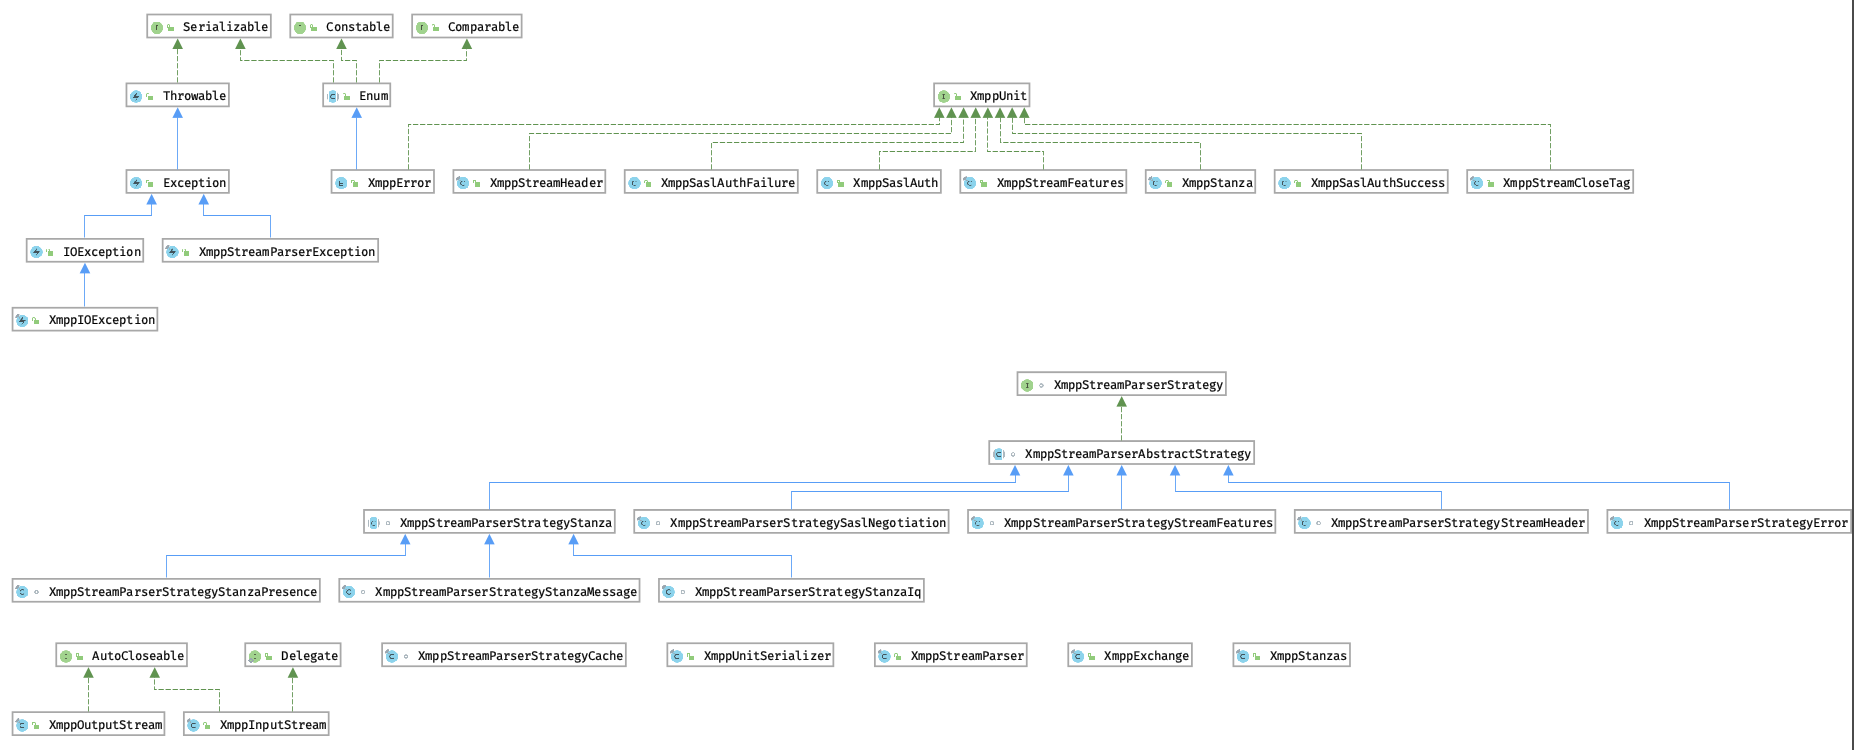
\includegraphics[width=1\textwidth]{core-classes}
	\caption{Диаграмма классов}
	\label{fig:core-classes}
\end{figure}

\begin{itemize}
	\item \code{Класс XmppInputStream} -- реализует Initial Stream для сервера и Response Stream для клиента
	\item \code{Класс XmppOutputStream} -- реализует Response Stream для сервера и Initial Stream для клиента
	\item \code{Класс XmppStanza} -- реализует и инкапсулирует в себе Stanza
	\item \code{Класс XmppStreamParser} -- парсер XMPP данных
	\item \code{Класс XmppUnitSerializer} -- сериализатор XMPP данных
\end{itemize}

\subsection{Серверная библиотека}

Серверная библиотека состоит из 1 класса: \code{BlockingXmppServer}. В нем реализовано сетевое взаимодействие между сервером и клиентами с помощью TCP-сокетов. В одном потоке происходит \code{accept} клиентских соединений. Затем взаимодействие в рамках каждого соединения осуществляется в новом потоке из пула потоков. Внутри используется ранее разработанная библиотека с реализацией протокола.

\subsection{Хранилище}

Хранилище реализовано в виде \code{java}-библиотеки. В нем реализованы классы и методы, которые инкапсулируют внутри себя SQL запросы к Postgres БД.

Схема БД представлена в скрипте в листинге

\lstinputlisting[caption={\code{Скрипт создания таблиц БД}},label={lst:db},language={sql}]{db/postgres/create.sql}

\subsection{Мессенжер}

Артефактом данного модуля является исполняемый java архив. Данный модуль использует серверную библиотеку и хранилище. 

Реализованы Stream Negotiation (установка соединения, авторизация методом PLAIN, биндинг ресурсов), отправка и получение сообщений (в том числе отложенных) и создание/чтение/изменение пользовательских ростеров.

Пользователи, их ростеры и сообщения хранятся в Postgres.

\section{Результаты тестирования}

Мессенжер был протестирован с помощью клиентского приложения Swift. Установка соединения, авторизация, чтение/обновление пользовательских ростеров, отправка и прием сообщений, отложенная доставка сообщений работают.

\section{Выводы}

В результате работы был изучен протокол \code{XMPP} на языке Java и была реализована его часть на языке Java в виде серверного приложения мессенжера. Реализованная функциональность была протестирована при взаимодействии с существующим клиентским приложением Swift. В будущем планируется реализовать механизм \code{Publish-Subscribe} для обмена сообщениями о присутствии и подписки и отказа от подписки на них.
Протокол XMPP хоть и не является новым, все еще является достаточно популярным и применяется в разных областях. Поэтому опыт разработки мессенжера был очень полезным для автора работы.

\section{Приложение. Исходный код}

\subsection{Реализация протокола XMPP -- модуль \code{core}}

\lstinputlisting[caption={\code{XmppStreamHeader.java}},label={lst:XmppStreamHeader}]{core/src/main/java/com/lamtev/xmpp/core/XmppStreamHeader.java}

\lstinputlisting[caption={\code{XmppStreamFeatures.java}},label={lst:XmppStreamFeatures}]{core/src/main/java/com/lamtev/xmpp/core/XmppStreamFeatures.java}

\lstinputlisting[caption={\code{XmppStreamCloseTag.java}},label={lst:XmppStreamCloseTag}]{core/src/main/java/com/lamtev/xmpp/core/XmppStreamCloseTag.java}

\lstinputlisting[caption={\code{XmppStanza.java}},label={lst:XmppStanza}]{core/src/main/java/com/lamtev/xmpp/core/XmppStanza.java}

\lstinputlisting[caption={\code{XmppSaslAuthSuccess.java}},label={lst:XmppSaslAuthSuccess}]{core/src/main/java/com/lamtev/xmpp/core/XmppSaslAuthSuccess.java}

\lstinputlisting[caption={\code{XmppSaslAuthFailure.java}},label={lst:XmppSaslAuthFailure}]{core/src/main/java/com/lamtev/xmpp/core/XmppSaslAuthFailure.java}

\lstinputlisting[caption={\code{XmppSaslAuth.java}},label={lst:XmppSaslAuth}]{core/src/main/java/com/lamtev/xmpp/core/XmppSaslAuth.java}

\lstinputlisting[caption={\code{XmppError.java}},label={lst:XmppError}]{core/src/main/java/com/lamtev/xmpp/core/XmppError.java}

\lstinputlisting[caption={\code{XmppExchange.java}},label={lst:XmppExchange}]{core/src/main/java/com/lamtev/xmpp/core/io/XmppExchange.java}

\lstinputlisting[caption={\code{XmppInputStream.java}},label={lst:XmppInputStream}]{core/src/main/java/com/lamtev/xmpp/core/io/XmppInputStream.java}

\lstinputlisting[caption={\code{XmppOutputStream.java}},label={lst:XmppOutputStream}]{core/src/main/java/com/lamtev/xmpp/core/io/XmppOutputStream.java}

\lstinputlisting[caption={\code{XmppStreamParser.java}},label={lst:XmppStreamParser}]{core/src/main/java/com/lamtev/xmpp/core/parsing/XmppStreamParser.java}

\lstinputlisting[caption={\code{XmppStreamParserStrategy.java}},label={lst:XmppStreamParserStrategy}]{core/src/main/java/com/lamtev/xmpp/core/parsing/XmppStreamParserStrategy.java}

\lstinputlisting[caption={\code{XmppStreamParserStrategyCache.java}},label={lst:XmppStreamParserStrategyCache}]{core/src/main/java/com/lamtev/xmpp/core/parsing/XmppStreamParserStrategyCache.java}

\lstinputlisting[caption={\code{XmppStreamParserAbstractStrategy.java}},label={lst:XmppStreamParserAbstractStrategy}]{core/src/main/java/com/lamtev/xmpp/core/parsing/XmppStreamParserAbstractStrategy.java}

\lstinputlisting[caption={\code{XmppStreamParserStrategySaslNegotiation.java}},label={lst:XmppStreamParserStrategySaslNegotiation}]{core/src/main/java/com/lamtev/xmpp/core/parsing/XmppStreamParserStrategySaslNegotiation.java}

\lstinputlisting[caption={\code{XmppStreamParserStrategyStanza.java}},label={lst:XmppStreamParserStrategyStanza}]{core/src/main/java/com/lamtev/xmpp/core/parsing/XmppStreamParserStrategyStanza.java}

\lstinputlisting[caption={\code{XmppStreamParserStrategyStanzaIq.java}},label={lst:XmppStreamParserStrategyStanzaIq}]{core/src/main/java/com/lamtev/xmpp/core/parsing/XmppStreamParserStrategyStanzaIq.java}

\lstinputlisting[caption={\code{XmppStreamParserStrategyStanzaMessage.java}},label={lst:XmppStreamParserStrategyStanzaMessage}]{core/src/main/java/com/lamtev/xmpp/core/parsing/XmppStreamParserStrategyStanzaMessage.java}

\lstinputlisting[caption={\code{XmppStreamParserStrategyStanzaPresence.java}},label={lst:XmppStreamParserStrategyStanzaPresence}]{core/src/main/java/com/lamtev/xmpp/core/parsing/XmppStreamParserStrategyStanzaPresence.java}

\lstinputlisting[caption={\code{XmppStreamParserStrategyStreamHeader.java}},label={lst:XmppStreamParserStrategyStreamHeader}]{core/src/main/java/com/lamtev/xmpp/core/parsing/XmppStreamParserStrategyStreamHeader.java}

\lstinputlisting[caption={\code{XmppUnitSerializer.java}},label={lst:XmppUnitSerializer}]{core/src/main/java/com/lamtev/xmpp/core/serialization/XmppUnitSerializer.java}

\lstinputlisting[caption={\code{XmppStanzas.java}},label={lst:XmppStanzas}]{core/src/main/java/com/lamtev/xmpp/core/util/XmppStanzas.java}

\subsection{Библиотека сервер -- модуль \code{server}}

\lstinputlisting[caption={\code{XmppServer.java}},label={lst:XmppServer}]{server/src/main/java/com/lamtev/xmpp/server/api/XmppServer.java}

\lstinputlisting[caption={\code{BlockingXmppServer.java}},label={lst:BlockingXmppServer}]{server/src/main/java/com/lamtev/xmpp/server/api/BlockingXmppServer.java}

\subsection{Хранилище -- модуль \code{db}}

\lstinputlisting[caption={\code{DBStorage.java}},label={lst:DBStorage}]{db/src/main/java/com/lamtev/xmpp/db/DBStorage.java}

\lstinputlisting[caption={\code{UserStorage.java}},label={lst:UserStorage}]{db/src/main/java/com/lamtev/xmpp/db/UserStorage.java}

\lstinputlisting[caption={\code{RosterStorage.java}},label={lst:RosterStorage}]{db/src/main/java/com/lamtev/xmpp/db/RosterStorage.java}

\lstinputlisting[caption={\code{MessageStorage.java}},label={lst:MessageStorage}]{db/src/main/java/com/lamtev/xmpp/db/MessageStorage.java}

\subsection{Мессенжер -- модуль \code{messenger}}

\lstinputlisting[caption={\code{Messenger.java}},label={lst:Messenger}]{messenger/src/main/java/com/lamtev/xmpp/messenger/Messenger.java}

\lstinputlisting[caption={\code{UserHandler.java}},label={lst:UserHandler}]{messenger/src/main/java/com/lamtev/xmpp/messenger/UserHandler.java}

\lstinputlisting[caption={\code{AuthBase64LoginPasswordExtractor.java}},label={lst:AuthBase64LoginPasswordExtractor}]{messenger/src/main/java/com/lamtev/xmpp/messenger/utils/AuthBase64LoginPasswordExtractor.java}

\lstinputlisting[caption={\code{StringGenerator.java}},label={lst:StringGenerator}]{messenger/src/main/java/com/lamtev/xmpp/messenger/utils/StringGenerator.java}

\end{document}
